% !TeX program = xelatex
\ifdefined\BookMaster\else
\documentclass[11pt,oneside]{article}
% !TeX program = xelatex
\usepackage[b5paper,left=22mm,right=22mm,top=20mm,bottom=22mm,footskip=11mm]{geometry}
\usepackage{fontspec}
\setmainfont{TeX Gyre Termes}
\setsansfont{TeX Gyre Heros}
\usepackage{amsmath,amssymb,mathtools,amsthm}
\renewcommand{\cdots}{\mathinner{\cdotp\cdotp\cdotp}}
\usepackage{graphicx,adjustbox,array,booktabs,longtable,multirow,enumitem,changepage,needspace}
\usepackage[table]{xcolor}
\usepackage{fancyhdr}
\raggedbottom
\interfootnotelinepenalty=10000
\newcommand{\BookFootnote}[2]{\begingroup\renewcommand{\thefootnote}{\fnsymbol{footnote}}\footnote[#1]{#2}\endgroup}
\newcommand{\BookFootnoteMark}[1]{\begingroup\renewcommand{\thefootnote}{\fnsymbol{footnote}}\footnotemark[#1]\endgroup}
\newcommand{\BookFootnoteText}[2]{\begingroup\renewcommand{\thefootnote}{\fnsymbol{footnote}}\footnotetext[#1]{#2}\endgroup}
\newenvironment{BookFloat}[1]{\par\addvspace{.6\baselineskip}\noindent\def\BookFloatID{#1}\begin{minipage}{\linewidth}\phantomsection\label{bookfloat:#1:start}}{\phantomsection\label{bookfloat:\BookFloatID:end}\end{minipage}\par\addvspace{.6\baselineskip}}

\usepackage[unicode,hidelinks]{hyperref}
\pagestyle{fancy}
\fancyhf{}
\newcommand{\BookFooter}{}
\fancyfoot[L]{\parbox[b]{\dimexpr\textwidth-15mm}{\footnotesize\BookFooter}}
\fancyfoot[R]{\footnotesize\thepage}
\renewcommand{\headrulewidth}{0pt}
\renewcommand{\footrulewidth}{0pt}
\setlength{\parindent}{0pt}
\setlength{\parskip}{0.2em}
\setlength{\emergencystretch}{3em}
\setlist{nosep,leftmargin=1.7em,labelsep=.65em}
\newif\ifBookNarrative
\BookNarrativetrue
\newenvironment{BookBody}{\setlength{\parindent}{0pt}}{}
\newcommand{\BookStatement}[1]{\par\addvspace{.6\baselineskip}\noindent #1\enspace\ignorespaces}
\newcommand{\BookLabel}[1]{\par\addvspace{.6\baselineskip}\needspace{3\baselineskip}\noindent\textbf{#1}\quad\ignorespaces}
\newcommand{\BookHeading}[1]{\par\addvspace{\baselineskip}\needspace{4\baselineskip}\noindent{\large\bfseries #1}\par\medskip}
\newcommand{\BookSubheading}[1]{\par\addvspace{.7\baselineskip}\needspace{3\baselineskip}\noindent{\bfseries #1}\par\smallskip}
\newcommand{\BookTextHeading}[1]{\par\addvspace{.7\baselineskip}\needspace{3\baselineskip}\noindent #1\par\smallskip}
\newcommand{\BookSectionTitle}[2]{\par\addvspace{1.2\baselineskip}\needspace{5\baselineskip}\noindent\colorbox{gray!25}{\sffamily\bfseries\small SECTION #1}\quad{\large\bfseries #2}\par\medskip}
\newcommand{\BookExerciseTitle}[1]{\par\addvspace{\baselineskip}\needspace{4\baselineskip}\noindent{\color{gray}\rule{1.5mm}{1.5mm}}\enspace{\large\bfseries Exercises #1}\par\medskip}
\newcommand{\BookBullet}[1]{\begin{list}{\textbullet}{\setlength{\leftmargin}{1.7em}\setlength{\labelwidth}{1em}\setlength{\labelsep}{.7em}\setlength{\topsep}{0pt}\setlength{\parsep}{0pt}\setlength{\itemsep}{0pt}}\item #1\end{list}}
\newcommand{\BookExercise}[2]{\begin{list}{\textbf{#1}}{\setlength{\leftmargin}{2.2em}\setlength{\labelwidth}{1.5em}\setlength{\labelsep}{.7em}\setlength{\topsep}{.15em}\setlength{\parsep}{0pt}\setlength{\itemsep}{0pt}}\item #2\end{list}}
\newcommand{\BookEnd}[1]{\unskip\nobreak\hfill\ensuremath{#1}}
\newcommand{\BookSource}[2]{\phantomsection\label{sourcepage:#1}} % Source-page anchors, retained through reflow.
\usepackage{multicol}
\usepackage{tikz}
\newcommand{\BookPartEntry}[2]{\par\noindent\makebox[17mm][l]{\bfseries Section #1}#2\par}
\newcommand{\BookPartTitle}[3]{\par\bigskip\noindent\begin{tikzpicture}\node[anchor=north west,inner sep=0pt,outer sep=0pt] (bookpart) at (0,0) {\begin{minipage}{\dimexpr\linewidth-.5pt}\hspace*{26mm}\begin{minipage}[t]{\dimexpr\linewidth-26mm}\begin{adjustbox}{max width=\linewidth}{\fontsize{20}{24}\selectfont\bfseries #2}\end{adjustbox}\par\vspace{6mm}\hrule\vspace{6mm}{\sffamily\footnotesize\setlength{\parskip}{.3em}#3}\vspace{3mm}\end{minipage}\end{minipage}};\path[shade,top color=gray!60,bottom color=white] (0,0) rectangle ([xshift=24mm]bookpart.south west);\node[anchor=north,font=\sffamily\bfseries\small] at (12mm,-2mm) {PART};\node[anchor=north,font=\sffamily\bfseries\Huge] at (12mm,-7mm) {#1};\end{tikzpicture}\par\bigskip}
\newsavebox{\BookMathBox}
\makeatletter
\newcommand{\BookInline}[1]{\leavevmode\hskip0pt\relax\begingroup\in@{\begin}{#1}\ifin@\sbox{\BookMathBox}{\(#1\)}\ifdim\wd\BookMathBox>\dimexpr\linewidth-1em\relax\resizebox{\dimexpr\linewidth-1em\relax}{!}{\usebox{\BookMathBox}}\else\(#1\)\fi\else\in@{\left}{#1}\ifin@\sbox{\BookMathBox}{\(#1\)}\ifdim\wd\BookMathBox>\dimexpr\linewidth-1em\relax\resizebox{\dimexpr\linewidth-1em\relax}{!}{\usebox{\BookMathBox}}\else\(#1\)\fi\else\(#1\)\fi\fi\endgroup\hskip0pt\relax}
\makeatother
\DeclareMathOperator{\Aut}{Aut}
\DeclareMathOperator{\End}{End}
\DeclareMathOperator{\Hom}{Hom}
\DeclareMathOperator{\GF}{GF}
\DeclareMathOperator{\irr}{irr}
\DeclareMathOperator{\lt}{lt}
\DeclareMathOperator{\lp}{lp}
\providecommand{\textcircled}[1]{\textnormal{(#1)}}

\begin{document}
\fi
\renewcommand{\BookFooter}{Section 30 Homomorphisms and Factor Rings}
\pdfbookmark[0]{Section 30 Homomorphisms and Factor Rings}{30_homomorphisms_and_factor_rings}
\ifdefined\BookMaster\else\setcounter{page}{243}\fi
% Source PDF page 260; original printed page 243
\BookSource{260}{243}
\BookNarrativetrue

\begin{BookBody}

\BookSectionTitle{30}{Homomorphisms and Factor Rings}

\BookTextHeading{\textbf{Factor Rings}  }

\noindent In Section 12 we investigated which subgroups of a given groups could be used to form a factor group. In this section we wish to do an analogous construction on a ring to form a factor ring. We start with an example.

\BookLabel{30.1 Example} For any \BookInline{n\in \mathbb{Z},\allowbreak n\mathbb{Z}} is a subring of \BookInline{\mathbb{Z}.} Thinking of \BookInline{\mathbb{Z}} as an abelian group, we know that \BookInline{n\mathbb{Z}} is a normal subgroup of \BookInline{\mathbb{Z}.} As we have seen\BookInline{,\allowbreak \mathbb{Z}/n\mathbb{Z}= \{a+ n\mathbb{Z}\mid a\in \mathbb{Z}\}} forms a group using addition defined by adding coset representatives. Furthermore\BookInline{,\allowbreak \mathbb{Z}/n\mathbb{Z}} is a ring where multiplication is defined by

\begin{center}\begin{adjustbox}{max width=\linewidth}\BookInline{\displaystyle (a+ n\mathbb{Z})(b+ n\mathbb{Z})= ab+ n\mathbb{Z}.}\end{adjustbox}\end{center}

\noindent We check that this multiplication is well defined. Let \BookInline{a^{\prime }\in a+ n\mathbb{Z}} and \BookInline{b^{\prime }\in b+ n\mathbb{Z}.} Then \BookInline{a^{\prime }= a+ nk} and \BookInline{b^{\prime }= b+ nr} for some integers \BookInline{k} and \BookInline{r.} Thus

\begin{center}\begin{adjustbox}{max width=\linewidth}\BookInline{\displaystyle \begin{aligned}a^{\prime }b^{\prime }&= (a+ nk)(b+ nr) \\ &= ab+ n(kb+ knr)+ anr \\ &= ab+ n(kb+ knr+ ar) \\ &\in ab+ n\mathbb{Z}.\end{aligned}}\end{adjustbox}\end{center}

\noindent From this calculation we see that regardless of which representatives from \BookInline{a+ n\mathbb{Z}} and \BookInline{b+ n\mathbb{Z}} we pick, our product is in the coset \BookInline{ab+ n\mathbb{Z}.} So we have a well-defined multiplication on the cosets of \BookInline{n\mathbb{Z}.}\BookEnd{\blacktriangle}

\end{BookBody}

% Source PDF page 261; original printed page 244
\BookSource{261}{244}
\BookNarrativetrue

\begin{BookBody}

\noindent Looking at the second line of the above computation, we can see that what was needed to verify \BookInline{a^{\prime }b^{\prime }\in ab+ n\mathbb{Z}} is that \BookInline{n(kb+ knr)+ anr\in n\mathbb{Z}.} The key to make this computation work is that when an element of \BookInline{\mathbb{Z}} is multiplied by an element of \BookInline{n\mathbb{Z},\allowbreak } the product is in \BookInline{n\mathbb{Z}.} This observation is the reason for the following definition.

\BookLabel{30.2 Definition} An additive subgroup \BookInline{N} of the ring \BookInline{R} is an\textbf{ ideal} if

\begin{center}\begin{adjustbox}{max width=\linewidth}\BookInline{\displaystyle aN= \{an\mid n\in N\}\subseteq N\;\text{and}\;Na= \{na\mid n\in N\}\subseteq N\;\text{for all}\;a\in R.}\end{adjustbox}\end{center} \BookEnd{\blacksquare}

\BookLabel{30.3 Example} We see that \BookInline{n\mathbb{Z}} is an ideal in the ring \BookInline{\mathbb{Z}} since we know it is a subring, and \BookInline{s(nm)= } \BookInline{(nm)s= n(ms)\in n\mathbb{Z}} for all \BookInline{s\in \mathbb{Z}.}\BookEnd{\blacktriangle}

\BookLabel{30.4 Example} Let \BookInline{F} be the ring of all functions mapping \BookInline{\mathbb{R}} into \BookInline{\mathbb{R},\allowbreak } and let \BookInline{C} be the subring of \BookInline{F} consisting of all the constant functions in \BookInline{F.} Is \BookInline{C} an ideal in \BookInline{F}? Why?

\BookLabel{\textit{Solution}} It is not true that the product of a constant function with every function is again a constant function. For example, the product of sin \BookInline{x} and 2 is the function 2 sin \BookInline{x.} Thus \BookInline{C} is not an ideal of \BookInline{F.}\BookEnd{\blacktriangle}

\BookTextHeading{\ensuremath{\blacksquare} \textbf{HISTORICAL NOTE}  }

\noindent It was Ernst Eduard Kummer (1810–1893) who introduced the concept of an “ideal complex number” in 1847 in order to preserve the notion of unique factorization in certain rings of algebraic integers. In particular, Kummer wanted to be able to factor into primes numbers of the form \BookInline{a_{0}+ a_{1}\alpha + a_{2}\alpha ^{2}+ \cdots + a_{p- 1}\alpha ^{p- 1},\allowbreak } where \BookInline{\alpha } is a complex root of \BookInline{x^{p}= 1(p} prime) and the \BookInline{a_{i}} are ordinary integers. Kummer had noticed that the naive definition of primes as “unfactorable numbers” does not lead to the expected results; the product of two such “unfactorable” numbers may well be divisible by other “unfactorable” numbers. Kummer defined “ideal prime factors” and “ideal numbers” in terms of certain congruence relationships; these “ideal factors” were then used as the divisors necessary to preserve unique factorization. By use of these, Kummer was in fact able to prove certain cases of Fermat’s Last Theorem, which states that \BookInline{x^{n}+ y^{n}= z^{n}} has no solutions \BookInline{x,\allowbreak y,\allowbreak z\in \mathbb{Z}^{+ }} if \BookInline{n>2.}

It turned out that an “ideal number,” which was in general not a “number” at all, was uniquely determined by the set of integers it “divided.” Richard Dedekind took advantage of this fact to identify the ideal factor with this set; he therefore called the set itself an ideal, and proceeded to show that it satisfied the definition given in the text. Dedekind was then able to define the notions of prime ideal and product of two ideals and show that any ideal in the ring of integers of any algebraic number field could be written uniquely as a product of prime ideals.

\BookLabel{30.5 Example} Let \BookInline{F} be as in the preceding example, and let \BookInline{N} be the subring of all functions \BookInline{f} such that \BookInline{f(2)= 0.} Is \BookInline{N} an ideal in \BookInline{F}? Why or why not?

\BookLabel{\textit{Solution}} Let \BookInline{f\in N} and let \BookInline{g\in F.} Then \BookInline{(fg)(2)= f(2)g(2)= 0g(2)= 0,\allowbreak } so \BookInline{fg\in N.} Similarly, we find that \BookInline{gf\in N.} Therefore \BookInline{N} is an ideal of \BookInline{F.}\BookEnd{\blacktriangle}

\BookLabel{30.6 Theorem} \textbf{(Analogue of Theorem 12.7)} Let \BookInline{H} be an additive subgroup of the ring \BookInline{R.} Multiplication of additive cosets of \BookInline{H} is well defined by the equation

\begin{center}\begin{adjustbox}{max width=\linewidth}\BookInline{\displaystyle (a+ H)(b+ H)= ab+ H}\end{adjustbox}\end{center}

\noindent if and only if \BookInline{H} is an ideal in \BookInline{R.}

\end{BookBody}

% Source PDF page 262; original printed page 245
\BookSource{262}{245}
\BookNarrativetrue

\begin{BookBody}

\BookLabel{\textit{Proof}} Suppose first that \BookInline{H} is an ideal in \BookInline{R.} Let \BookInline{a,\allowbreak b\in R,\allowbreak a^{\prime }\in a+ H,\allowbreak } and \BookInline{b^{\prime }\in b+ H.} There are elements \BookInline{h_{1},\allowbreak h_{2}\in H} with \BookInline{a^{\prime }= a+ h_{1}} and \BookInline{b^{\prime }= b+ h_{2}.} We have

\begin{center}\begin{adjustbox}{max width=\linewidth}\BookInline{\displaystyle \begin{aligned}a^{\prime }b^{\prime }&= (a+ h_{1})(b+ h_{2}) \\ &= ab+ ah_{2}+ h_{1}b+ h_{1}h_{2} \\ &\in ab+ H\;\text{since}\;H\;\text{is an ideal}\;.\end{aligned}}\end{adjustbox}\end{center}

\noindent We now suppose that \BookInline{(a+ H)(b+ H)= ab+ H} defines a binary operation on cosets of \BookInline{H} in \BookInline{R.} We let \BookInline{a\in R} and \BookInline{h\in H} with the goal of showing that \BookInline{aH\subseteq H} and \BookInline{Ha\subseteq H.} Since \BookInline{h+ H= 0+ H,\allowbreak }

\begin{center}\begin{adjustbox}{max width=\linewidth}\BookInline{\displaystyle H= 0a+ H= (0+ H)(a+ H)= (h+ H)(a+ H)= ha+ H.}\end{adjustbox}\end{center}

\noindent This shows \BookInline{ha\in H,\allowbreak } which implies \BookInline{Ha\subseteq H.} Similarly,

\begin{center}\begin{adjustbox}{max width=\linewidth}\BookInline{\displaystyle H= a0+ H= (a+ H)(0+ H)= (a+ H)(h+ H)= ah+ H.}\end{adjustbox}\end{center}

\noindent This shows \BookInline{ah\in H} and therefore \BookInline{aH\subseteq H.} Thus \BookInline{H} is an ideal in \BookInline{R.} \BookEnd{\blacklozenge}

Once we know that multiplication by choosing representatives is well defined on additive cosets of a subring \BookInline{N} of \BookInline{R,\allowbreak } the associative law for multiplication and the distributive laws for these cosets follow immediately from the same properties in \BookInline{R.} We have at once this corollary of Theorem 30.6.

\BookLabel{30.7 Corollary} \textbf{(Analogue of Corollary 12.8)} Let \BookInline{N} be an ideal of a ring \BookInline{R.} Then the additive cosets of \BookInline{N} form a ring \BookInline{R/N} with the binary operations defined by

\begin{center}\begin{adjustbox}{max width=\linewidth}\BookInline{\displaystyle (a+ N)+ (b+ N)= (a+ b)+ N}\end{adjustbox}\end{center}

\noindent and

\begin{center}\begin{adjustbox}{max width=\linewidth}\BookInline{\displaystyle (a+ N)(b+ N)= ab+ N.}\end{adjustbox}\end{center} \BookEnd{\blacklozenge}

\BookLabel{30.8 Definition} The ring \BookInline{R/N} in the preceding corollary is the\textbf{ factor ring} (or\textbf{ quotient ring})\textbf{ of} \BookInline{R} \textbf{by} \BookInline{N.}\BookEnd{\blacksquare}

If we use the term\textit{ quotient ring}, be sure not to confuse it with the notion of the \BookInline{\text{fi}eld} \textit{of quotients} of an integral domain, discussed in Section 26.

\BookTextHeading{\textbf{Homomorphisms}}

\noindent We defined the concepts of\textit{ homomorphism} and\textit{ isomorphism} for rings in Section 22, since we wished to talk about evaluation homomorphisms for polynomials and about isomorphic rings. We repeat some definitions here for easy reference. Recall that a homomorphism is a\textit{ structure-relating map}. A homomorphism for rings must relate both their additive structure and their multiplicative structure.

\BookLabel{30.9 Definition} A map \BookInline{\phi } of a ring \BookInline{R} into a ring \BookInline{R^{\prime }} is a\textbf{ homomorphism} if

\begin{center}\begin{adjustbox}{max width=\linewidth}\BookInline{\displaystyle \phi (a+ b)= \phi (a)+ \phi (b)}\end{adjustbox}\end{center}

\noindent and

\begin{center}\begin{adjustbox}{max width=\linewidth}\BookInline{\displaystyle \phi (ab)= \phi (a)\phi (b)}\end{adjustbox}\end{center}

\noindent for all elements \BookInline{a} and \BookInline{b} in \BookInline{R.} \BookEnd{\blacksquare}

In Example 22.10 we defined evaluation homomorphisms, and Example 22.11 showed that the map \BookInline{\phi:\mathbb{Z}\to \mathbb{Z}_{n},\allowbreak } where \BookInline{\phi (m)} is the remainder of \BookInline{m} when divided 
% Source PDF page 263; original printed page 246
\BookSource{263}{246}
by \BookInline{n,\allowbreak } is a homomorphism. We give another simple but very fundamental example of a homomorphism.

\end{BookBody}

\BookNarrativetrue

\begin{BookBody}

\BookLabel{30.10 Example} \textbf{(Projection Homomorphisms)} Let \BookInline{R_{1},\allowbreak R_{2},\allowbreak \cdots,\allowbreak R_{n}} be rings. For each \BookInline{i,\allowbreak } the map \BookInline{\pi _{i}:} \BookInline{R_{1}\times R_{2}\times \cdots \times R_{n}\to R_{i}} defined by \BookInline{\pi _{i}(r_{1},\allowbreak r_{2},\allowbreak \cdots,\allowbreak r_{n})= r_{i}} is a homomorphism,\textit{ pro}\textit{jection onto the} \BookInline{ith} \textit{component}. The two required properties of a homomorphism hold for \BookInline{\pi _{i}} since both addition and multiplication in the direct product are computed by addition and multiplication in each individual component\BookInline{.}\BookEnd{\blacktriangle}

\BookTextHeading{\textbf{Properties of Homomorphisms}  }

\noindent We continue to parallel our development of ring homomorphisms and factor rings with the analogous material for group homomorphisms and factor groups.

\BookLabel{30.11 Theorem} Let \BookInline{\phi:R\to R^{\prime }} be a ring homomorphism.

\BookExercise{1.}{If 0 is the additive identity in \BookInline{R,\allowbreak } then \BookInline{\phi (0)= 0^{\prime }} is the additive identity in \BookInline{R^{\prime }.}}

\BookExercise{2.}{If \BookInline{a\in R,\allowbreak } then \BookInline{\phi (- a)= - \phi (a).}}

\BookExercise{3.}{If \BookInline{S} is a subring of \BookInline{R,\allowbreak } then \BookInline{\phi [S]} is a subring of \BookInline{R^{\prime }.}}

\BookExercise{4.}{If \BookInline{S^{\prime }} is a subring of \BookInline{R^{\prime },\allowbreak } then \BookInline{\phi ^{- 1}[S^{\prime }]} is a subring of \BookInline{R.}}

\BookExercise{5.}{If \BookInline{R} has unity 1, then \BookInline{\phi (1)} is unity for \BookInline{\phi [R].}}

\BookExercise{6.}{If \BookInline{N} is an ideal in \BookInline{R,\allowbreak } then \BookInline{\phi [N]} is an ideal in \BookInline{\phi [R].}}

\BookExercise{7.}{If \BookInline{N^{\prime }} is an ideal in either \BookInline{R^{\prime }} or \BookInline{\phi [R],\allowbreak } then \BookInline{\phi ^{- 1}[N^{\prime }]} is an ideal in \BookInline{R.}}

\BookLabel{\textit{Proof}} Let \BookInline{\phi } be a homomorphism of a ring \BookInline{R} into a ring \BookInline{R^{\prime }.} Since, in particular\BookInline{,\allowbreak \phi } can be viewed as a group homomorphism of \BookInline{\langle R,\allowbreak + \rangle } into \BookInline{\langle R^{\prime },\allowbreak + ^{\prime }\rangle,\allowbreak } Theorem 8.5 tells us that \BookInline{\phi (0)= 0^{\prime }} is the additive identity element of \BookInline{R^{\prime }} and that \BookInline{\phi (- a)= - \phi (a).}

Theorem 8.5 also tells us that if \BookInline{S} is a subring of \BookInline{R,\allowbreak } then, considering the additive group \BookInline{\langle S,\allowbreak + \rangle,\allowbreak } the set \BookInline{\langle \phi [S],\allowbreak + ^{\prime }\rangle } gives a subgroup of \BookInline{\langle R^{\prime },\allowbreak + ^{\prime }\rangle.} If \BookInline{\phi (s_{1})} and \BookInline{\phi (s_{2})} are two elements of \BookInline{\phi [S],\allowbreak } then

\begin{center}\begin{adjustbox}{max width=\linewidth}\BookInline{\displaystyle \phi (s_{1})\phi (s_{2})= \phi (s_{1}s_{2})}\end{adjustbox}\end{center}

\noindent and \BookInline{\phi (s_{1}s_{2})\in \phi [S].} Thus \BookInline{\phi (s_{1})\phi (s_{2})\in \phi [S],\allowbreak } so \BookInline{\phi [S]} is closed under multiplication. Consequently\BookInline{,\allowbreak \phi [S]} is a subring of \BookInline{R^{\prime }.}

Going the other way, Theorem 8.5 also shows that if \BookInline{S^{\prime }} is a subring of \BookInline{R^{\prime },\allowbreak } then \BookInline{\langle \phi ^{- 1}[S^{\prime }],\allowbreak + \rangle } is a subgroup of \BookInline{\langle R,\allowbreak + \rangle.} Let \BookInline{a,\allowbreak b\in \phi ^{- 1}[S^{\prime }],\allowbreak } so that \BookInline{\phi (a)\in S^{\prime }} and \BookInline{\phi (b)\in S^{\prime }.} Then

\begin{center}\begin{adjustbox}{max width=\linewidth}\BookInline{\displaystyle \phi (ab)= \phi (a)\phi (b).}\end{adjustbox}\end{center}

\noindent Since \BookInline{\phi (a)\phi (b)\in S^{\prime },\allowbreak } we see that \BookInline{ab\in \phi ^{- 1}[S^{\prime }],\allowbreak } so \BookInline{\phi ^{- 1}[S^{\prime }]} is closed under multiplication and thus is a subring of \BookInline{R.}

If \BookInline{R} has unity 1, then for all \BookInline{r\in R,\allowbreak }

\begin{center}\begin{adjustbox}{max width=\linewidth}\BookInline{\displaystyle \phi (r)= \phi (1r)= \phi (r1)= \phi (1)\phi (r)= \phi (r)\phi (1),\allowbreak }\end{adjustbox}\end{center}

\noindent so \BookInline{\phi (1)} is unity for \BookInline{\phi [R].}

The proof of the remainder of the theorem is Exercise 22. \BookEnd{\blacklozenge}

Note in Theorem 30.11 that \BookInline{\phi (1)} is unity for \BookInline{\phi [R],\allowbreak } but not necessarily for \BookInline{R^{\prime }} as we ask you to illustrate in Exercise 9. Furthermore, although \BookInline{\phi [N]} is an ideal in \BookInline{\phi [R],\allowbreak } it may not be an ideal in \BookInline{R^{\prime }} as verified in Exercise 22.

\end{BookBody}

% Source PDF page 264; original printed page 247
\BookSource{264}{247}
\BookNarrativetrue

\begin{BookBody}

\BookLabel{30.12 Definition} Let a map \BookInline{\phi:R\to R^{\prime }} be a homomorphism of rings. The subring

\begin{center}\begin{adjustbox}{max width=\linewidth}\BookInline{\displaystyle \phi ^{- 1}[0^{\prime }]= \{r\in R\mid \phi (r)= 0^{\prime }\}}\end{adjustbox}\end{center}

\noindent is the\textbf{ kernel} of \BookInline{\phi,\allowbreak } denoted by Ker\BookInline{(\phi ).} \BookEnd{\blacksquare}

If we forget about the multiplicative part of a ring, we see that the kernel of a ring homomorphism is the same as the kernel of the underlying group homomorphism. Any property of a group homomorphism must also hold for a ring homomorphism.

\BookLabel{30.13 Theorem} \textbf{Analogue of Theorem 10.17} Let \BookInline{\phi:R_{1}\to R_{2}} be a ring homomorphism. The elements \BookInline{a,\allowbreak b\in R_{1}} are in the same additive coset of Ker\BookInline{(\phi )} if and only if \BookInline{\phi (a)= \phi (b)}\BookEnd{\blacklozenge}

\BookLabel{30.14 Theorem} \textbf{Analogue of Corollary 10.19} A ring homomorphism \BookInline{\phi:R_{1}\to R_{2}} is one-to-one if and only if Ker\BookInline{(\phi )= \{0\}.}\BookEnd{\blacklozenge}

\noindent The kernel of a group homomorphism \BookInline{\phi:G_{1}\to G_{2}} is a normal subgroup of \BookInline{G_{1}} and normality is what is needed in order to construct a factor group from a subgroup. The situation is similar in rings. We need a subring to be an ideal in order to construct a factor ring. The following theorem states that in fact the kernel of a ring homomorphism is an ideal.

\BookLabel{30.15 Theorem} Let \BookInline{\phi:R_{1}\to R_{2}} be a ring homomorphism. Then Ker\BookInline{(\phi )} is an ideal in \BookInline{R_{1}.}

\BookLabel{\textit{Proof}} Since \BookInline{\{0\}\subset R_{2}} is an ideal in \BookInline{R_{2},\allowbreak } Ker\BookInline{(\phi )= \phi ^{- 1}[\{0\}]} is an ideal in \BookInline{R_{1}} by Property 7 of Theorem \BookInline{30.11.}\BookEnd{\blacklozenge}

\BookTextHeading{\textbf{Fundamental Homomorphism Theorem}  }

\noindent To complete our analogy with groups, we give the analogues of Theorems 12.12 and 12.14.

\BookLabel{30.16 Theorem} \textbf{(Analogue of Theorem 12.12)} Let \BookInline{N} be an ideal of a ring \BookInline{R.} Then \BookInline{\gamma:R\to R/N} given by \BookInline{\gamma (x)= x+ N} is a ring homomorphism with kernel \BookInline{N.}

\BookLabel{\textit{Proof}} The additive part is done in Theorem 12.12. Turning to the multiplicative question, we see that

\begin{center}\begin{adjustbox}{max width=\linewidth}\BookInline{\displaystyle \gamma (xy)= (xy)+ N= (x+ N)(y+ N)= \gamma (x)\gamma (y).}\end{adjustbox}\end{center} \BookEnd{\blacklozenge}

\BookLabel{30.17 Theorem} \textbf{(Fundamental Homomorphism Theorem; Analogue of Theorem 12.14)} Let \BookInline{\phi:} \BookInline{R\to R^{\prime }} be a ring homomorphism with kernel \BookInline{N.} Then \BookInline{\phi [R]} is a ring, and the map \BookInline{\mu:R/N\to \phi [R]} given by \BookInline{\mu (x+ N)= \phi (x)} is an isomorphism. If \BookInline{\gamma:R\to R/N} is the homomorphism given by \BookInline{\gamma (x)= x+ N,\allowbreak } then for each \BookInline{x\in R,\allowbreak } we have \BookInline{\phi (x)= \mu \circ \gamma (x).}

\begin{BookFloat}{30_homomorphisms_and_factor_rings-p264-17}
\begin{center}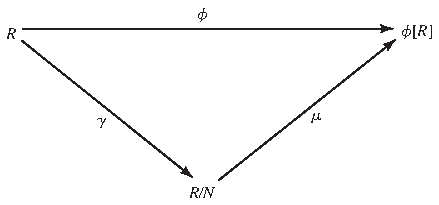
\includegraphics[width=0.602\linewidth,height=.8\textheight,keepaspectratio]{assets/p264_16.pdf}\end{center}
\begin{center}\small\textbf{30.18 Figure}\end{center}
\end{BookFloat}

\end{BookBody}

% Source PDF page 265; original printed page 248
\BookSource{265}{248}
\BookNarrativetrue

\begin{BookBody}

\BookLabel{\textit{Proof}} This follows at once from Theorems 30.15 and 30.16. Figure 30.18 is the analogue of Fig\BookInline{.12.15.}\BookEnd{\blacklozenge}

\BookLabel{30.19 Example} Example 30.3 shows that \BookInline{n\mathbb{Z}} is an ideal of \BookInline{\mathbb{Z},\allowbreak } so we can form the factor ring \BookInline{\mathbb{Z}/n\mathbb{Z}.} Example 22.11 shows that \BookInline{\phi:\mathbb{Z}\to \mathbb{Z}_{n}} where \BookInline{\phi (m)} is the remainder of \BookInline{m} modulo \BookInline{n} is a homomorphism, and we see that Ker\BookInline{(\phi )= n\mathbb{Z}.} Theorem 30.17 then shows that the map \BookInline{\mu:\mathbb{Z}/n\mathbb{Z}\to \mathbb{Z}_{n}} where \BookInline{\mu (m+ n\mathbb{Z})} is the remainder of \BookInline{m} modulo \BookInline{n} is well defined and is an isomorphism\BookInline{.}\BookEnd{\blacktriangle}

\BookLabel{30.20 Example} Continuing Example 30.5, let \BookInline{F} be the ring of all functions mapping \BookInline{\mathbb{R}} into \BookInline{\mathbb{R}} and let \BookInline{N} be the subset of \BookInline{F} consisting of all functions \BookInline{f} with \BookInline{f(2)= 0.} The set \BookInline{N} is an ideal in \BookInline{F,\allowbreak } so \BookInline{F/N} is a ring. Furthermore\BookInline{,\allowbreak N} is the kernel of the evaluation homomorphism \BookInline{\phi _{2}:F\to \mathbb{R}} defined by \BookInline{\phi _{2}(f)= f(2).} Since \BookInline{\phi _{2}} maps onto \BookInline{\mathbb{R},\allowbreak F/N} is isomorphic with \BookInline{\mathbb{R}} by Theorem 30.17. The function \BookInline{\mu:F/N\to \mathbb{R}} given by \BookInline{\mu (f)= f(2)} is an isomorphism. \BookEnd{\blacktriangle}

In summary, every ring homomorphism with domain \BookInline{R} gives rise to a factor ring \BookInline{R/N,\allowbreak } and every factor ring \BookInline{R/N} gives rise to a homomorphism mapping \BookInline{R} into \BookInline{R/N.} An \textit{ideal} in ring theory is analogous to a\textit{ normal subgroup} in the group theory. Both are the type of substructure needed to form a factor structure.

\end{BookBody}

\BookNarrativefalse

\begin{BookBody}

\BookExerciseTitle{30}

\BookTextHeading{\textbf{Computations}}

\BookExercise{1.}{Describe all ring homomorphisms of \BookInline{\mathbb{Z}\times \mathbb{Z}} into \BookInline{\mathbb{Z}\times \mathbb{Z}.[}\textit{Hint:} Note that if \BookInline{\phi } is such a homomorphism, then \BookInline{\phi ((1,\allowbreak 0))= \phi ((1,\allowbreak 0))\phi ((1,\allowbreak 0))} and \BookInline{\phi ((0,\allowbreak 1))= \phi ((0,\allowbreak 1))\phi ((0,\allowbreak 1)).} Consider also \BookInline{\phi ((1,\allowbreak 0)(0,\allowbreak 1)).]}}

\BookExercise{2.}{Find all positive integers \BookInline{n} such that \BookInline{\mathbb{Z}_{n}} contains a subring isomorphic to \BookInline{\mathbb{Z}_{2}.}}

\BookExercise{3.}{Find all ideals \BookInline{N} of \BookInline{\mathbb{Z}_{12}.} In each case compute \BookInline{\mathbb{Z}_{12}/N;} that is, find a known ring to which the quotient ring is isomorphic.}

\BookExercise{4.}{Give addition and multiplication tables for \BookInline{2\mathbb{Z}/8\mathbb{Z}.} Are \BookInline{2\mathbb{Z}/8\mathbb{Z}} and \BookInline{\mathbb{Z}_{4}} isomorphic rings?}

\BookTextHeading{\textbf{Concepts}}

\noindent In Exercises 5 through 7, correct the definition of the italicized term without reference to the text, if correction is needed, so that it is in a form acceptable for publication.

\BookExercise{5.}{An\textit{ isomorphism of} \BookInline{a} \textit{ring} \BookInline{R} with a ring \BookInline{R^{\prime }} is a homomorphism \BookInline{\phi:R\to R^{\prime }} such that Ker\BookInline{(\phi )= \{0\}.}}

\BookExercise{6.}{An\textit{ ideal} \BookInline{N} of a ring \BookInline{R} is an additive subgroup of \BookInline{\langle R,\allowbreak + \rangle } such that for all \BookInline{r\in R} and all \BookInline{n\in N,\allowbreak } we have \BookInline{rn\in N} and \BookInline{nr\in N.}}

\BookExercise{7.}{The\textit{ kernel of} \BookInline{a} \textit{homomorphism} \BookInline{\phi } mapping a ring \BookInline{R} into a ring \BookInline{R^{\prime }} is \BookInline{\{\phi (r)= 0^{\prime }\mid r\in R\}.}}

\BookExercise{8.}{Let \BookInline{F} be the ring of all functions mapping \BookInline{\mathbb{R}} into \BookInline{\mathbb{R}} and having derivatives of all orders. Differentiation gives a map \BookInline{\delta:F\to F} where \BookInline{\delta (f(x))= f^{\prime }(x).} Is \BookInline{\delta } a homomorphism? Why? Give the connection between this exercise and Example 30.4.}

\BookExercise{9.}{Give an example of a ring homomorphism \BookInline{\phi:R\to R^{\prime }} where \BookInline{R} has unity 1 and \BookInline{\phi (1)\neq 0^{\prime },\allowbreak } but \BookInline{\phi (1)} is not unity for \BookInline{R^{\prime }.}}

\BookExercise{10.}{Determine whether each of the following is true or false.}

\BookExercise{a.}{The concept of a ring homomorphism is closely connected with the idea of a factor ring.}

\BookExercise{b.}{A ring homomorphism \BookInline{\phi:R\to R^{\prime }} carries ideals of \BookInline{R} into ideals of \BookInline{R^{\prime }.}}

\BookExercise{c.}{A ring homomorphism is one-to-one if and only if the kernel is \BookInline{\{0\}.}}

\BookExercise{d.}{\textbf{d}\BookInline{.\mathbb{Q}} is an ideal in \BookInline{\mathbb{R}.}}

\end{BookBody}

% Source PDF page 266; original printed page 249
\BookSource{266}{249}
\BookNarrativefalse

\begin{BookBody}

\BookExercise{e.}{Every ideal in a ring is a subring of the ring.}

\BookExercise{f.}{Every subring of every ring is an ideal of the ring.}

\BookExercise{g.}{Every quotient ring of every commutative ring is again a commutative ring.}

\BookExercise{h.}{The rings \BookInline{\mathbb{Z}/4\mathbb{Z}} and \BookInline{\mathbb{Z}_{4}} are isomorphic.}

\BookExercise{i.}{An ideal \BookInline{N} in a ring \BookInline{R} with unity 1 is all of \BookInline{R} if and only if \BookInline{1\in N.}}

\BookExercise{j.}{The concept of an ideal is to the concept of a ring as the concept of a normal subgroup is to the concept of a group.}

\BookExercise{11.}{Let \BookInline{R} be a ring. Observe that \BookInline{\{0\}} and \BookInline{R} are both ideals of \BookInline{R.} Are the factor rings \BookInline{R/R} and \BookInline{R/\{0\}} of real interest? Why?}

\BookExercise{12.}{Give an example to show that a factor ring of an integral domain may be a field.}

\BookExercise{13.}{Give an example to show that a factor ring of an integral domain may have divisors of 0.}

\BookExercise{14.}{Give an example to show that a factor ring of a ring with divisors of 0 may be an integral domain.}

\BookExercise{15.}{Find a subring of the ring \BookInline{\mathbb{Z}\times \mathbb{Z}} that is not an ideal of \BookInline{\mathbb{Z}\times \mathbb{Z}.}}

\BookExercise{16.}{A student is asked to prove that a quotient ring of a ring \BookInline{R} modulo an ideal \BookInline{N} is commutative if and only if \BookInline{(rs- sr)\in N} for all \BookInline{r,\allowbreak s\in R.} The student starts out:}

Assume \BookInline{R/N} is commutative. Then \BookInline{rs= sr} for all \BookInline{r,\allowbreak s\in R/N.}

\BookExercise{a.}{Why does the instructor reading this expect an incorrect proof?}

\BookExercise{b.}{What should the student have written?}

\BookExercise{c.}{Prove the assertion. (Note the “if and only if.”)}

\BookTextHeading{\textbf{Theory}}

\BookInline{\Big[\Big]}

\BookExercise{17.}{Let \BookInline{R= \{a+ b\sqrt{2}\mid a,\allowbreak b\in \mathbb{Z}\}} and let \BookInline{R^{\prime }} consist of all \BookInline{2\times 2} matrices of the form \BookInline{\begin{bmatrix} a & 2b \\ b & a \end{bmatrix}} for \BookInline{a,\allowbreak b\in \mathbb{Z}.} Show that \BookInline{R} is a subring of \BookInline{\mathbb{R}} and that \BookInline{R^{\prime }} is a subring of \BookInline{M_{2}(\mathbb{Z}).} Then show that \BookInline{\phi:R\to R^{\prime },\allowbreak } where \BookInline{\phi (a+ b\sqrt{2})= } \BookInline{\begin{bmatrix} a & 2b \\ b & a \end{bmatrix}} is an isomorphism.}

\BookExercise{18.}{Show that each homomorphism from a field to a ring is either one-to-one or maps everything onto 0.}

\BookExercise{19.}{Show that if \BookInline{R,\allowbreak R^{\prime },\allowbreak } and \BookInline{R^{\prime \prime }} are rings, and if \BookInline{\phi:R\to R^{\prime }} and \BookInline{\psi:R^{\prime }\to R^{\prime \prime }} are homomorphisms, then the composite function \BookInline{\psi \phi:R\to R^{\prime \prime }} is a homomorphism. (See Exercise 39 of Section 8.)}

\BookExercise{20.}{Let \BookInline{R} be a commutative ring with unity of prime characteristic \BookInline{p.} Show that the map \BookInline{\phi _{p}:R\to R} given by \BookInline{\phi _{p}(a)= a^{p}} is a homomorphism (the\textbf{ Frobenius homomorphism}).}

\BookExercise{21.}{Let \BookInline{R} and \BookInline{R^{\prime }} be rings and let \BookInline{\phi:R\to R^{\prime }} be a ring homomorphism such that \BookInline{\phi [R]\neq \{0^{\prime }\}.} Show that if \BookInline{R} has unity 1 and \BookInline{R^{\prime }} has no 0 divisors, then \BookInline{\phi (1)} is unity for \BookInline{R^{\prime }.}}

\BookExercise{22.}{Let \BookInline{\phi:R\to R^{\prime }} be a ring homomorphism and let \BookInline{N} be an ideal of \BookInline{R.}}

\BookExercise{a.}{Show that \BookInline{\phi [N]} is an ideal of \BookInline{\phi [R].}}

\BookExercise{b.}{Give an example to show that \BookInline{\phi [N]} need not be an ideal of \BookInline{R^{\prime }.}}

\BookExercise{c.}{Let \BookInline{N^{\prime }} be an ideal either of \BookInline{\phi [R]} or of \BookInline{R^{\prime }.} Show that \BookInline{\phi ^{- 1}[N^{\prime }]} is an ideal of \BookInline{R.}}

\BookExercise{23.}{Let \BookInline{F} be a field, and let \BookInline{S} be any subset of \BookInline{F\times F\times \cdots \times F} for \BookInline{n} factors. Show that the set \BookInline{N_{S}} of all \BookInline{f(x_{1},\allowbreak \cdots,\allowbreak x_{n})\in F[x_{1},\allowbreak \cdots,\allowbreak x_{n}]} that have every element \BookInline{(a_{1},\allowbreak \cdots,\allowbreak a_{n})} of \BookInline{S} as a zero (see Exercise 28 of Section 27) is an ideal in \BookInline{F[x_{1},\allowbreak \cdots,\allowbreak x_{n}].} This is of importance in algebraic geometry.}

\BookExercise{24.}{Show that a factor ring of a field is either the trivial (zero) ring of one element or is isomorphic to the field.}

\BookExercise{25.}{Show that if \BookInline{R} is a ring with unity and \BookInline{N} is an ideal of \BookInline{R} such that \BookInline{N\neq R,\allowbreak } then \BookInline{R/N} is a ring with unity.}

\BookExercise{26.}{Let \BookInline{R} be a commutative ring and let \BookInline{a\in R.} Show that \BookInline{I_{a}= \{x\in R\mid } \textit{ax} \BookInline{= 0\}} is an ideal of \BookInline{R.}}

\BookExercise{27.}{Show that an intersection of ideals of a ring \BookInline{R} is again an ideal of \BookInline{R.}}

\BookExercise{28.}{Let \BookInline{R} and \BookInline{R^{\prime }} be rings and let \BookInline{N} and \BookInline{N^{\prime }} be ideals of \BookInline{R} and \BookInline{R^{\prime },\allowbreak } respectively. Let \BookInline{\phi } be a homomorphism of \BookInline{R} into \BookInline{R^{\prime }.} Show that \BookInline{\phi } induces a natural homomorphism \BookInline{\phi _{\ast }:R/N\to R^{\prime }/N^{\prime }} if \BookInline{\phi [N]\subseteq N^{\prime }.(}Use Exercise 41 of Section 12.)}

\end{BookBody}

% Continuation on source PDF page 267, preceding Section 31
\BookNarrativefalse

\begin{BookBody}

\BookExercise{29.}{Let \BookInline{\phi } be a homomorphism of a ring \BookInline{R} with unity onto a nonzero ring \BookInline{R^{\prime }.} Let \BookInline{u} be a unit in \BookInline{R.} Show that \BookInline{\phi (u)} is a unit in \BookInline{R^{\prime }.}}

\BookExercise{30.}{An element \BookInline{a} of a ring \BookInline{R} is\textbf{ nilpotent} if \BookInline{a^{n}= 0} for some \BookInline{n\in \mathbb{Z}^{+ }.} Show that the collection of all nilpotent elements in a commutative ring \BookInline{R} is an ideal, the\textbf{ nilradical of} \BookInline{R.}}

\BookExercise{31.}{Referring to the definition given in Exercise 30, find the nilradical of the ring \BookInline{\mathbb{Z}_{12}} and observe that it is one of the ideals of \BookInline{\mathbb{Z}_{12}} found in Exercise 3. What is the nilradical of \BookInline{\mathbb{Z}}? of \BookInline{\mathbb{Z}_{32}}?}

\BookExercise{32.}{Referring to Exercise 30, show that if \BookInline{N} is the nilradical of a commutative ring \BookInline{R,\allowbreak } then \BookInline{R/N} has as nilradical the trivial ideal \BookInline{\{0+ N\}.}}

\BookExercise{33.}{Let \BookInline{R} be a commutative ring and \BookInline{N} an ideal of \BookInline{R.} Referring to Exercise 30, show that if every element of \BookInline{N} is nilpotent and the nilradical of \BookInline{R/N} is \BookInline{R/N,\allowbreak } then the nilradical of \BookInline{R} is \BookInline{R.}}

\BookExercise{34.}{Let \BookInline{R} be a commutative ring and \BookInline{N} an ideal of \BookInline{R.} Show that the set \BookInline{\sqrt{N}} of all \BookInline{a\in R,\allowbreak } such that \BookInline{a^{n}\in N} for some \BookInline{n\in \mathbb{Z}^{+ },\allowbreak } is an ideal of \BookInline{R,\allowbreak } the\textbf{ radical of} \BookInline{N.}}

\BookExercise{35.}{Referring to Exercise 34, show by examples that for proper ideals \BookInline{N} of a commutative ring \BookInline{R,\allowbreak }}

\textbf{a}\BookInline{.\sqrt{N}} need not equal \BookInline{N} \textbf{b}\BookInline{.\sqrt{N}} may equal \BookInline{N.}

\BookExercise{36.}{What is the relationship of the ideal \BookInline{\sqrt{N}} of Exercise 34 to the nilradical of \BookInline{R/N(}see Exercise 30)? Word your answer carefully.}

\BookExercise{37.}{Show that \BookInline{\phi:\mathbb{C}\to M_{2}(\mathbb{R})} given by}

\begin{center}\begin{adjustbox}{max width=\linewidth}\BookInline{\displaystyle \phi(a + bi) = \begin{pmatrix} a & b \\ -b & a \end{pmatrix}}\end{adjustbox}\end{center}

for \BookInline{a,\allowbreak b\in \mathbb{R}} gives an isomorphism of \BookInline{\mathbb{C}} with the subring \BookInline{\phi [\mathbb{C}]} of \BookInline{M_{2}(\mathbb{R}).}

\end{BookBody}
\ifdefined\BookMaster\let\BookFinish\relax\else\def\BookFinish{\end{document}}\fi\BookFinish
